\section{المنهجية}
\label{sec:methodology}

نقترح طريقة إخفاء معلومات وفق نموذج الصندوق الأسود تخفي رسالة سرية داخل محادثة عامة.
لدى المرسل والمستقبل حسابان على منصة تواصل اجتماعي.
يبحث المرسل عن سلسلة نقاش، ويكتب ما يبدو تعليقًا أو ردًا عاديًا، ثم ينشره.
يقرأ المستقبل لاحقًا السلسلة نفسها، ويجد مساهمة المرسل، ويسترجع الحمولة المخفية.
تستخدم دراستنا بيانات على طراز \EN{Reddit} بوصفها الحالة الرئيسة.
يستهدف التصميم أي بيئة نقاش متسلسلة؛ أما ما إذا كان ينتقل بسلاسة إلى منصات أخرى فيبقى أمرًا لم يُختبر بعد.
يوضح الشكل~\ref{fig:end-to-end} السيناريو الخفي الكامل والافتراضات المشتركة اللازمة للمزامنة.

\begin{figure}[t]
	\centering
	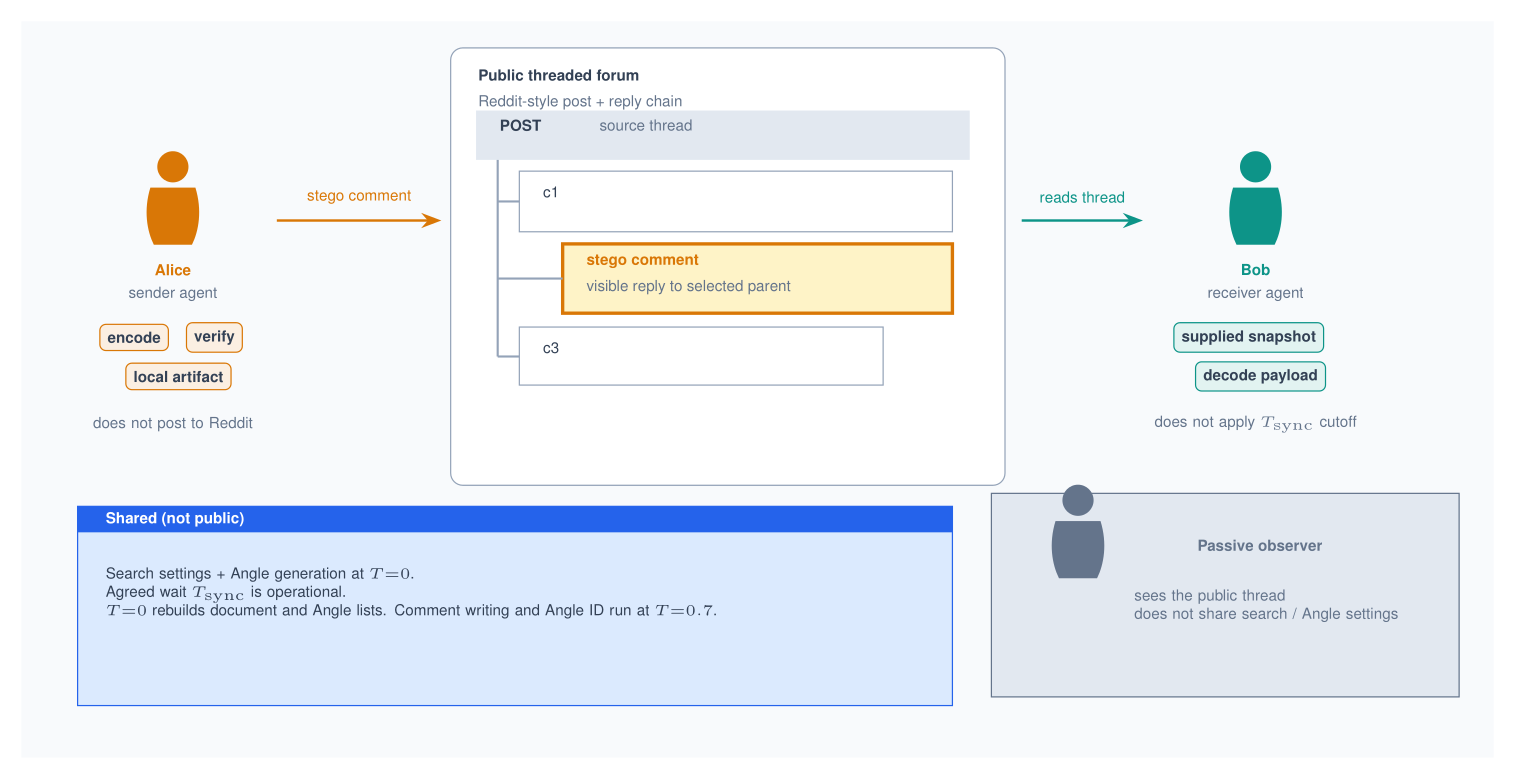
\includegraphics[width=0.78\linewidth]{figures/end_to_end_scenario.png}
	\caption{سيناريو الاتصال الخفي: يستخدم أليس وبوب قناة عامة متسلسلة؛ وتعتمد المزامنة على معاملات تشغيل مشتركة ونافذة زمنية متفق عليها.}
	\label{fig:end-to-end}
\end{figure}

\subsection{بنية النظام}
 يتمحور الإطار المقترح حول عملية تضمين متعددة الطبقات تستفيد من \textit{موضع الرد} و\textit{الموضوع الدلالي} للمحتوى بوصفهما حاملين للحمولة السرية. ومن خلال مقابلة البيانات الثنائية مع أفعال حوارية عالية المستوى، وتحديدًا اختيار هدف الرد واختيار \textit{وجهة نظر}، يحمل النظام الحمولة عبر قناة الانتقاء مع الحفاظ على الطبيعية الإدراكية في النص المرئي. وفي سير العمل المنفذ، يعيد المستقبل بناء سياق ما قبل المرسل نفسه، أي لقطة السلسلة والبحث الحتمي ووجهات النظر المعاد توليدها، ثم يفك ترميز فهارس الاختيار نفسها لاسترجاع الحمولة. يبين الشكل~\ref{fig:two-layer} طبقتي التضمين وتفاعلهما مع التوليد.

\subsection{المتطلبات التشغيلية}
لتحقيق المزامنة، يجب أن يحافظ المرسل والمستقبل على الوصول إلى:
\begin{itemize}
    \item \textbf{قناة اتصال عامة:} حسابات على منصة التواصل الاجتماعي المستهدفة.
    \item \textbf{معاملات تشغيل مشتركة:} خوارزمية بحث حتمية، وبيانات وصفية للمنشور، وقيود بحث معرّفة مسبقًا.
    \item \textbf{إعدادات إعادة بناء حتمية:} ضبط متزامن للنموذج أو الخلفية البرمجية في المراحل الحتمية، مثل \texttt{temperature=0}، كي يعيد الطرفان توليد مصطلحات البحث ومجموعة وجهات النظر نفسها من المدخلات نفسها.
    \item \textbf{نافذة زمنية متفق عليها:} مدة $T_{sync}$ متفاوض عليها تستخدم لترشيح حالة السلسلة بحيث يعيد المستقبل بناء سياق التعليقات نفسه الذي شاهده المرسل.
\end{itemize}

\subsection{حتمية البحث وإطار المزامنة}
\label{sec:search_determinism}
إن ضمان عمل أليس وبوب على مجموعة وثائق البحث نفسها هو حجر الأساس في فك الترميز الموثوق. فمرحلة البحث المنفذة سلسلة معالجة مسبقة قابلة للإعادة وليست بحثًا عشوائيًا على الويب. يولد مولد مصطلحات البحث أولًا بين 12 و20 استعلامًا فريدًا من عنوان المنشور ونصه ورابطه باستخدام نموذج سير العمل عند \texttt{temperature=0}. ثم ينفذ كل استعلام عبر واجهة \EN{Google Custom Search} بصيغة طلب ثابتة، \texttt{first=1} و\texttt{count=10}، وتحذف الروابط المكررة ونتائج \EN{PDF}، وتجلب الروابط الباقية على دفعات من ثلاثة. تستخدم مرحلة استخراج المحتوى موائمًا مبنيًا على \EN{crawl4ai} يزحف إلى الروابط ويستخرج النص الأساسي. وتخزن القائمة المسطحة الناتجة من نصوص الصفحات المجلوبة كمدونة نتائج بحث، كما يسجل خط المعالجة قيم تجزئة للتحقق من سلامة المصطلحات والمدونة كي يمكن إعادة تشغيل المدونة نفسها في المراحل اللاحقة. يلخص الشكل~\ref{fig:research-pipeline} سلسلة البحث الحتمية هذه.

\begin{figure*}[t]
	\centering
	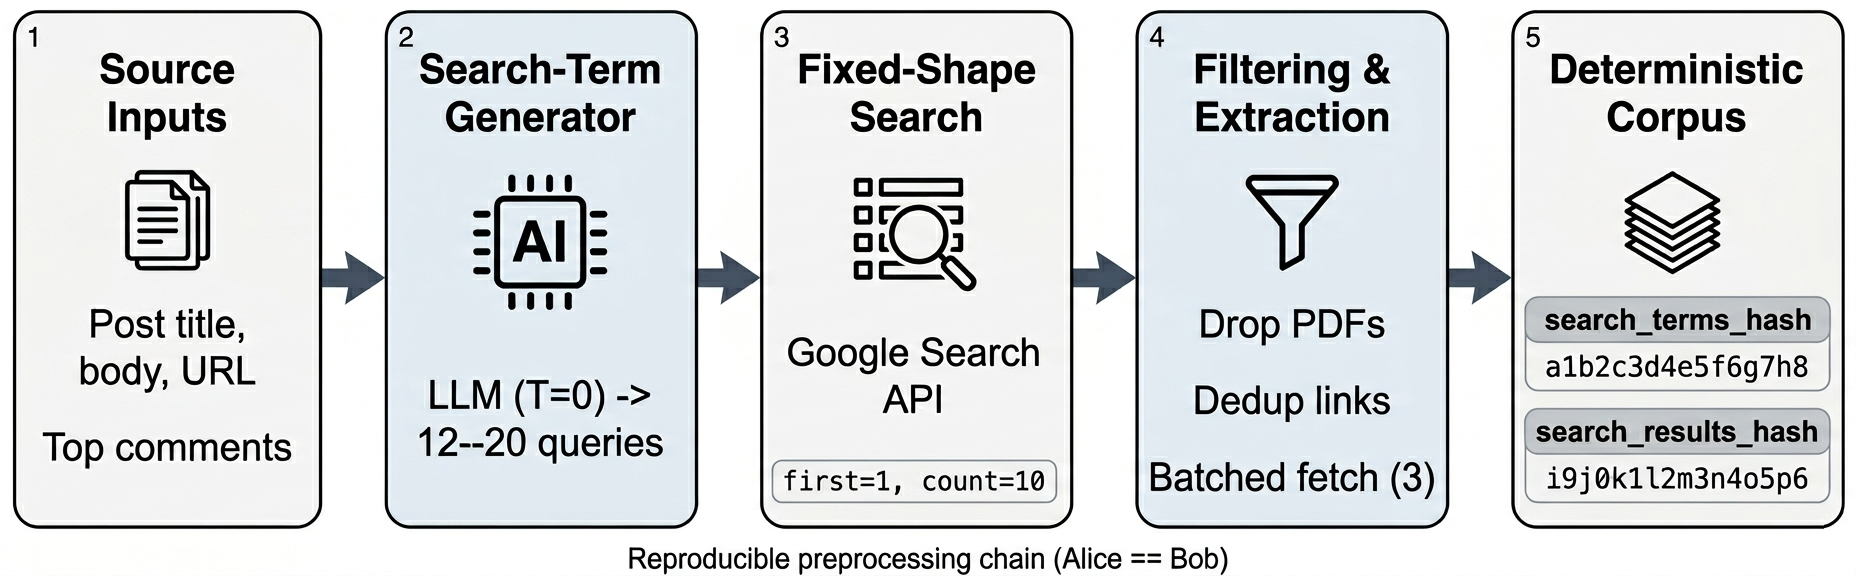
\includegraphics[width=\textwidth,height=0.62\textheight,keepaspectratio]{figures/research_pipeline_deterministic}
	\caption{مرحلة البحث الحتمية: توليد مشترك للمصطلحات، ومعاملات بحث ثابتة، وترشيح، وجلب دفعي، وقيم تجزئة للتحقق من سلامة مدونات قابلة للإعادة.}
	\label{fig:research-pipeline}
\end{figure*}

\subsection{مزامنة الحالة: النافذة الزمنية}
لضمان أن يرى أليس وبوب حالة متطابقة من شجرة المحادثة، يجب الالتزام بمدة نافذة زمنية متفق عليها $T_{sync}$. وتطبق آلية المزامنة هذه لمعالجة زمن المعالجة الكامن في وكيل المرسل:
\begin{enumerate}
    \item \textbf{جانب المرسل:} يلتقط أليس لقطة من سلسلة النقاش عند الزمن $t_{start}$، وينفذ التضمين متعدد الطبقات، ثم ينشر التعليق المُوَرّى المولد عند $t_{publish}$.
    \item \textbf{جانب المستقبل:} بعد تحديد المساهمة الإخفائية المنشورة عند $t_{publish}$، يرشح بوب الحالة التاريخية للسلسلة بحيث تشمل فقط التعليقات المنشأة قبل $t_{publish} - T_{sync}$.
\end{enumerate}
والمدة المتفق عليها $T_{sync}$ متطلب مزامنة خارجي: إذ يجب على المستقبل توفير لقطة سابقة للنشر أو تطبيق حد الزمن بنفسه قبل إعادة البناء. أما المستقبل الحالي فيحذف تعليق المرسل ويعيد البناء من المنشور المعطى، لكنه لا يفرض حد الزمن هذا من تلقاء نفسه. يبين الشكل~\ref{fig:tsync} النافذة الزمنية المقصودة نسبة إلى $t_{start}$ و$t_{publish}$.

\begin{figure*}[t]
	\centering
	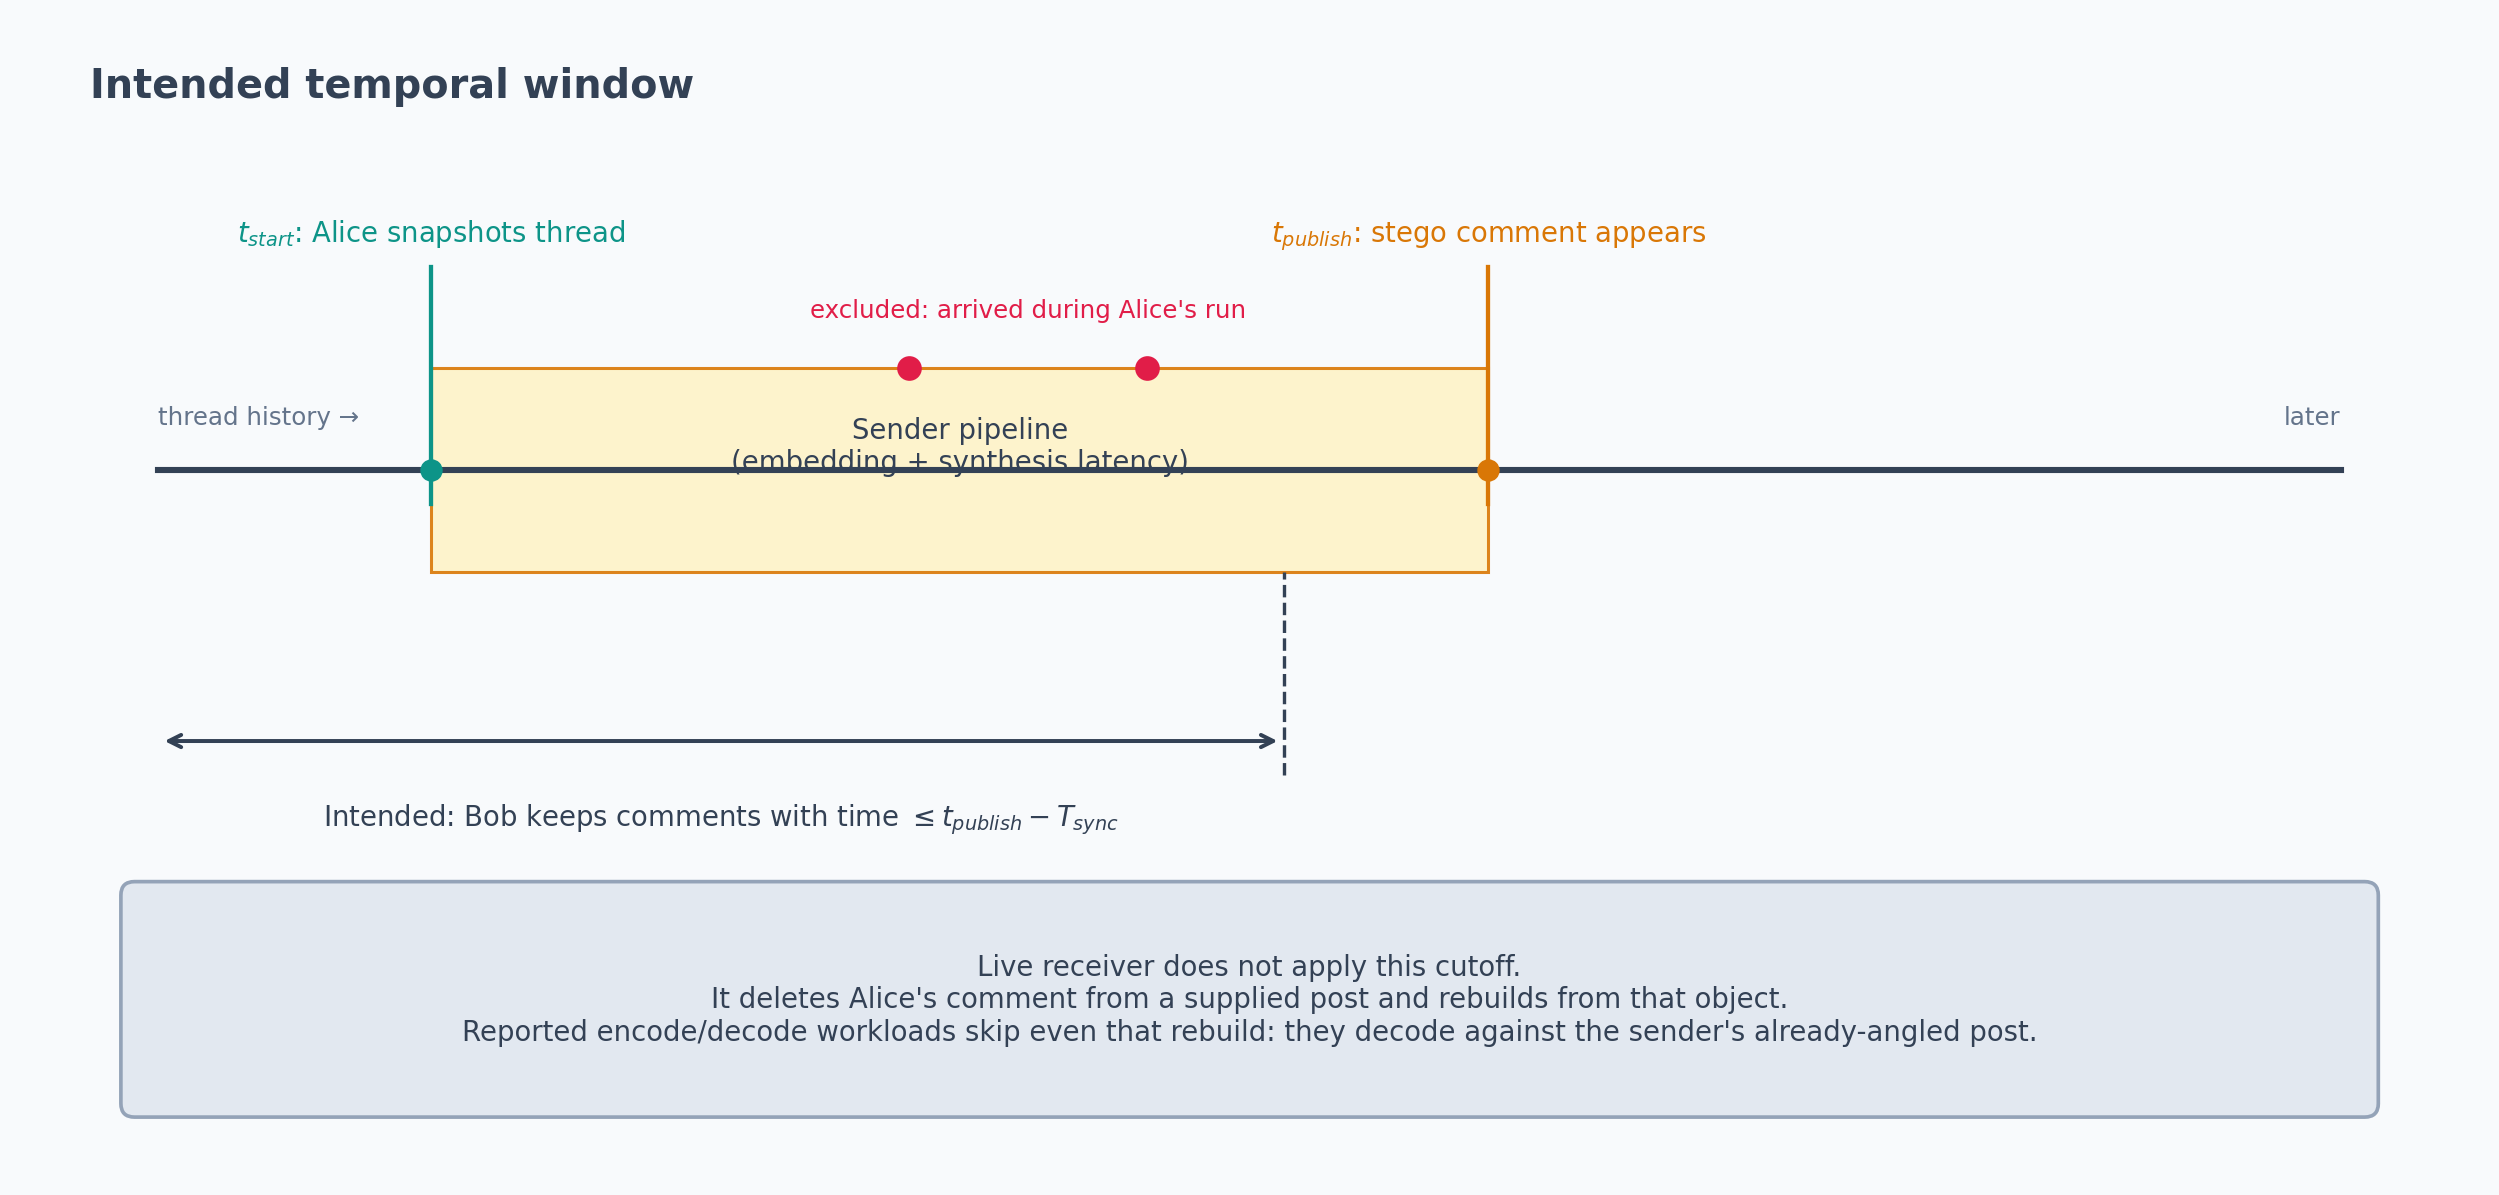
\includegraphics[width=\textwidth,height=0.58\textheight,keepaspectratio]{figures/temporal_sync_window}
	\caption{المزامنة الزمنية: تطابق حالة السلسلة المعاد بناؤها لدى بوب حالة أليس من خلال الاتفاق على $T_{sync}$ وترشيح التعليقات نسبة إلى $t_{publish}$.}
	\label{fig:tsync}
\end{figure*}

\subsection{تحضير الحمولة وضغطها}
\label{sec:compression}
قبل التضمين، تمر الحمولة بمرحلتين عكوسيتين: تحويل حماية اختياري، ثم ضاغط قائم على القاموس. وتنفذ المرحلتان مرة واحدة في وحدة ترميز واحدة يستدعيها المرسل والمستقبل مباشرة، لا نسختين منفصلتين قد تنحرفان عن بعضهما؛ أما ما فوق هذه الوحدة، أي خطا معالجة المرسل والمستقبل، فيقتصر على الدخل والخرج والتخزين المؤقت والتنسيق.

\subsubsection{تحويل الحماية}
يحدد التحويل بالضبط الإعدادي ويسجل في سجل تدقيق المرسل كي يعرف المستقبل أي معكوس يطبق. وثمة ثلاثة أنماط منفذة:
\begin{itemize}[leftmargin=*]
    \item \texttt{plain}، وهو الافتراضي: تمرر الحمولة دون تغيير.
    \item \texttt{hmac\_xor\_v1}: شيفرة تدفق. تولّد قيمة استخدام وحيد \EN{(nonce)} جديدة $N$ بطول 16 بايت مع سر مشترك مسبقًا $s$ تدفقَ مفتاح $K=\mathrm{HMAC}_s(N\Vert c_0)\Vert\mathrm{HMAC}_s(N\Vert c_1)\Vert\cdots$، حيث $c_i$ عداد بطول 4 بايتات بترتيب البايت الأكبر أولًا يمثل القيمة $i$، و\EN{SHA-256} دالة التجزئة طوال البناء. ثم تجرى عملية \EN{XOR} بين حمولة \EN{UTF-8} وتدفق المفتاح $K$. ويوثق الناتج بوسم \EN{HMAC} مبتور بطول 16 بايت محسوب على الوسم \EN{"swsec1"} متبوعًا بـ$N$ ثم النص المعمى؛ ويمنع هذا الوسم أي إثبات صحة تحت النمط \texttt{secure\_compact\_v2} عن طريق الخطأ. وتُرمّز قيمة الاستخدام الوحيد والنص المعمى والوسم كل على حدة بترميز \EN{Base64} الآمن للروابط، ثم توصل بنقاط في سلسلة واحدة.
    \item \texttt{secure\_compact\_v2}: البنية نفسها والوسم نفسه تحت الوسم \EN{"swsec2"}، غير أن الحمولة تضغط بـ\EN{zlib} قبل التعمية، وتسلسل الحقول الثلاثة الخام كبايتات قبل ترميز \EN{Base64}، فينتج ذلك كتلة واحدة أقصر بدلًا من ثلاثة حقول موصولة بنقاط.
\end{itemize}
ويجري التحقق من الوسم بزمن ثابت، ولا ينتج عن عدم التطابق أي حمولة بدلًا من حمولة تالفة، فلا يصدر المستقبل تخمينًا غير موثق. وتضيف هذه الطبقة السرية فوق القناة الخفية؛ وهي ليست ما يجعل القناة خفية.

\subsubsection{قاموس الجلسة}
يعمل الضاغط على قاموس مرتب $D=(d_1,\dots,d_{|D|})$ من كتل نصية تجمع بترتيب ثابت واحد: نص المنشور، ثم نص كل نتيجة بحث (نص الصفحة الكامل أو المقتطف، أيهما توفر)، ثم كل متن تعليق بالترتيب المسطح الحتمي. وهذا الترتيب مهم لأن فهارس القاموس موضعية: فإذا بنى الطرفان $D$ بطريقتين مختلفتين، أشار الفهرس نفسه صامتًا إلى نص مختلف عند كل منهما. ويمكن اختياريًا تفعيل ملف سعة يحد من عدد كتل نتائج البحث والتعليقات ويعيد ترتيبها أيضًا -- إذ يرتب مدخلات نتائج البحث والتعليقات ترتيبًا حتميًا ثم يوزعها بالتناوب -- وهو معطل افتراضيًا كي يتشارك الطرفان عادةً ترتيب المصادر الكامل غير المرتب الموصوف أعلاه.

\subsubsection{التجزئة المثلى بكلفة البتات}
ليكن $W(m)=\lceil\log_2(m+1)\rceil$ حين $m>0$ و$W(m)=0$ فيما عدا ذلك، دالةً تعطي العرض الثابت لحقل عديم الإشارة أكبر قيمة مقبولة فيه $m$، وليكن $L_{\max}=\max_j|d_j|$. تجزأ الحمولة إلى تسلسل من الرموز من النوعين المبينين في الجدول~\ref{tab:token-layout}.

\begin{table}[t]
\centering
\caption{بنية رموز سلسلة الحمولة المضغوطة. لكل حقل عرض ثابت بمعلومية $D$، غير أن فك الترميز تسلسلي بحت: يتعلق موضع بداية أي رمز بموضع نهاية الرمز الذي قبله، فلا تحمل السلسلة علامة مزامنة داخلية ولا يمكن استئناف قراءتها من إزاحة عشوائية.}
\label{tab:token-layout}
\small
\begin{tabularx}{\columnwidth}{@{}l X l@{}}
\toprule
الرمز & بنية الحقول & الكلفة بالبتات \\
\midrule
حرفي & \EN{\texttt{0}} $\Vert$ الطول $\ell$ (8 بتات) $\Vert$ بايتات \EN{UTF-8} & $9+8b$ \\
مرجعي & \EN{\texttt{1}} $\Vert$ الفهرس $j$ ($W(|D|)$) $\Vert$ الإزاحة ($W(|d_j|)$) $\Vert$ الطول ($W(L_{\max})$) & $1+W(|D|)+W(|d_j|)+W(L_{\max})$ \\
\bottomrule
\end{tabularx}
\end{table}

يقيد المقطع الحرفي بـ250 محرفًا، وهو ما يثبت عرض حقل طوله عند $W(250)=8$ بتات. ويعد هذا الحقل المحارف لا البايتات: يقرأ فاك الترميز مجموعات من 8 بتات حتى يفك بالضبط $\ell$ محرفًا، و$b$ أعلاه هو عدد بايتات \EN{UTF-8} الناتج عن ذلك. ولا يولد الرمز المرجعي إلا للتطابقات التي تبلغ ثلاثة محارف فأكثر، إذ تستبعد التطابقات الأقصر قبل أن تعمل البرمجة الديناميكية، لأن كلفة المؤشر فيها تفوق البايتات الحرفية التي كان سيحل محلها.

وبمعلومية هذه الكلف، تختار التجزئة ببرمجة ديناميكية رجعية على مواضع الحمولة،
\[
C(i)=\min_{t\in T(i)}\bigl(\mathrm{cost}(t)+C(i+|t|)\bigr),\qquad C(n)=0,
\]
حيث تضم $T(i)$ كل طول حرفي حتى الحد الأقصى، ولكل تكرار قاموسي يبدأ عند $i$ امتداده المتصل الأطول فقط -- إذ تحدد التكرارات بتمديد تطابق حرفي جشع لا بحصر كل طول وسيط ممكن. لذلك تكون البرمجة الديناميكية مثلى تمامًا على مجموعة المرشحين هذه، لا على كل تجزئة ممكنة للحمولة.

والسلسلة الصادرة هي راية نمط واحدة يتبعها تسلسل الرموز: تسبق الراية \EN{\texttt{1}} التجزئة المثلى، وتسبق الراية \EN{\texttt{0}} سلسلة بتات \EN{UTF-8} الخام. ويصدر الضاغط الراية \EN{\texttt{0}} كلما لم تكن التجزئة أقصر فعليًا من \EN{UTF-8} المجرد، وهو ما يحد أسوأ حالات التمدد ببت واحد. يعرض الشكل~\ref{fig:compression} بناء القاموس ونمطي الترميز.

\begin{figure*}[t]
	\centering
	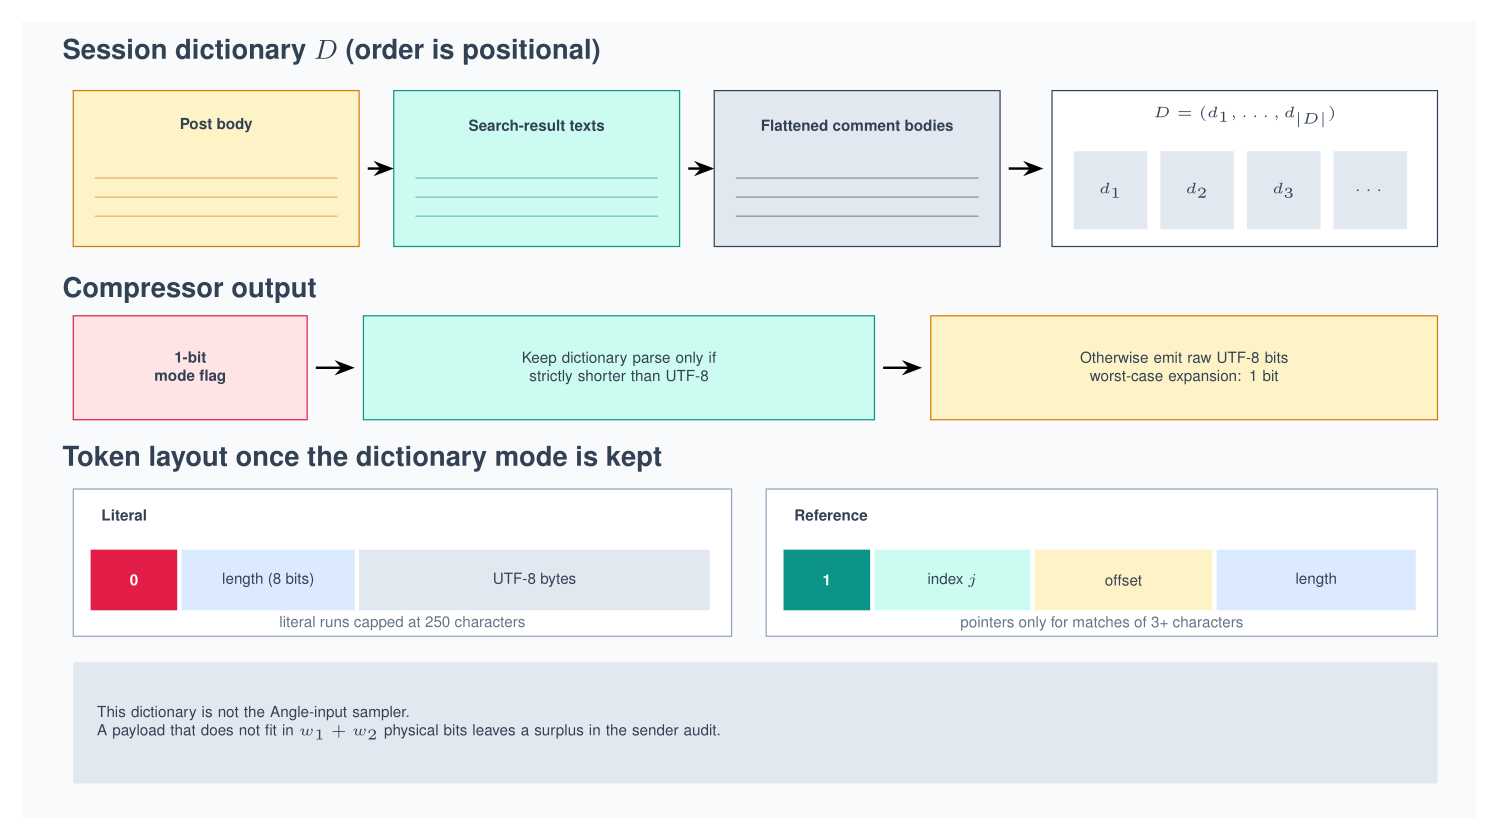
\includegraphics[width=\textwidth,height=0.62\textheight,keepaspectratio]{figures/payload_compression_dp}
	\caption{يبني ضغط الحمولة قاموسًا خاصًا بالجلسة من نصوص السلسلة والبحث، ثم يختار بين المقاطع الحرفية والمقاطع المشفرة بالقاموس لتقليل كلفة البتات.}
	\label{fig:compression}
\end{figure*}

\subsection{بنية التضمين الدلالي ثنائية الطبقة}
يعطي الشكل~\ref{fig:two-layer} نظرة تخطيطية إلى كيفية تقسيم طبقتي التضمين للحمولة قبل التوليد.

\begin{figure*}[t]
	\centering
	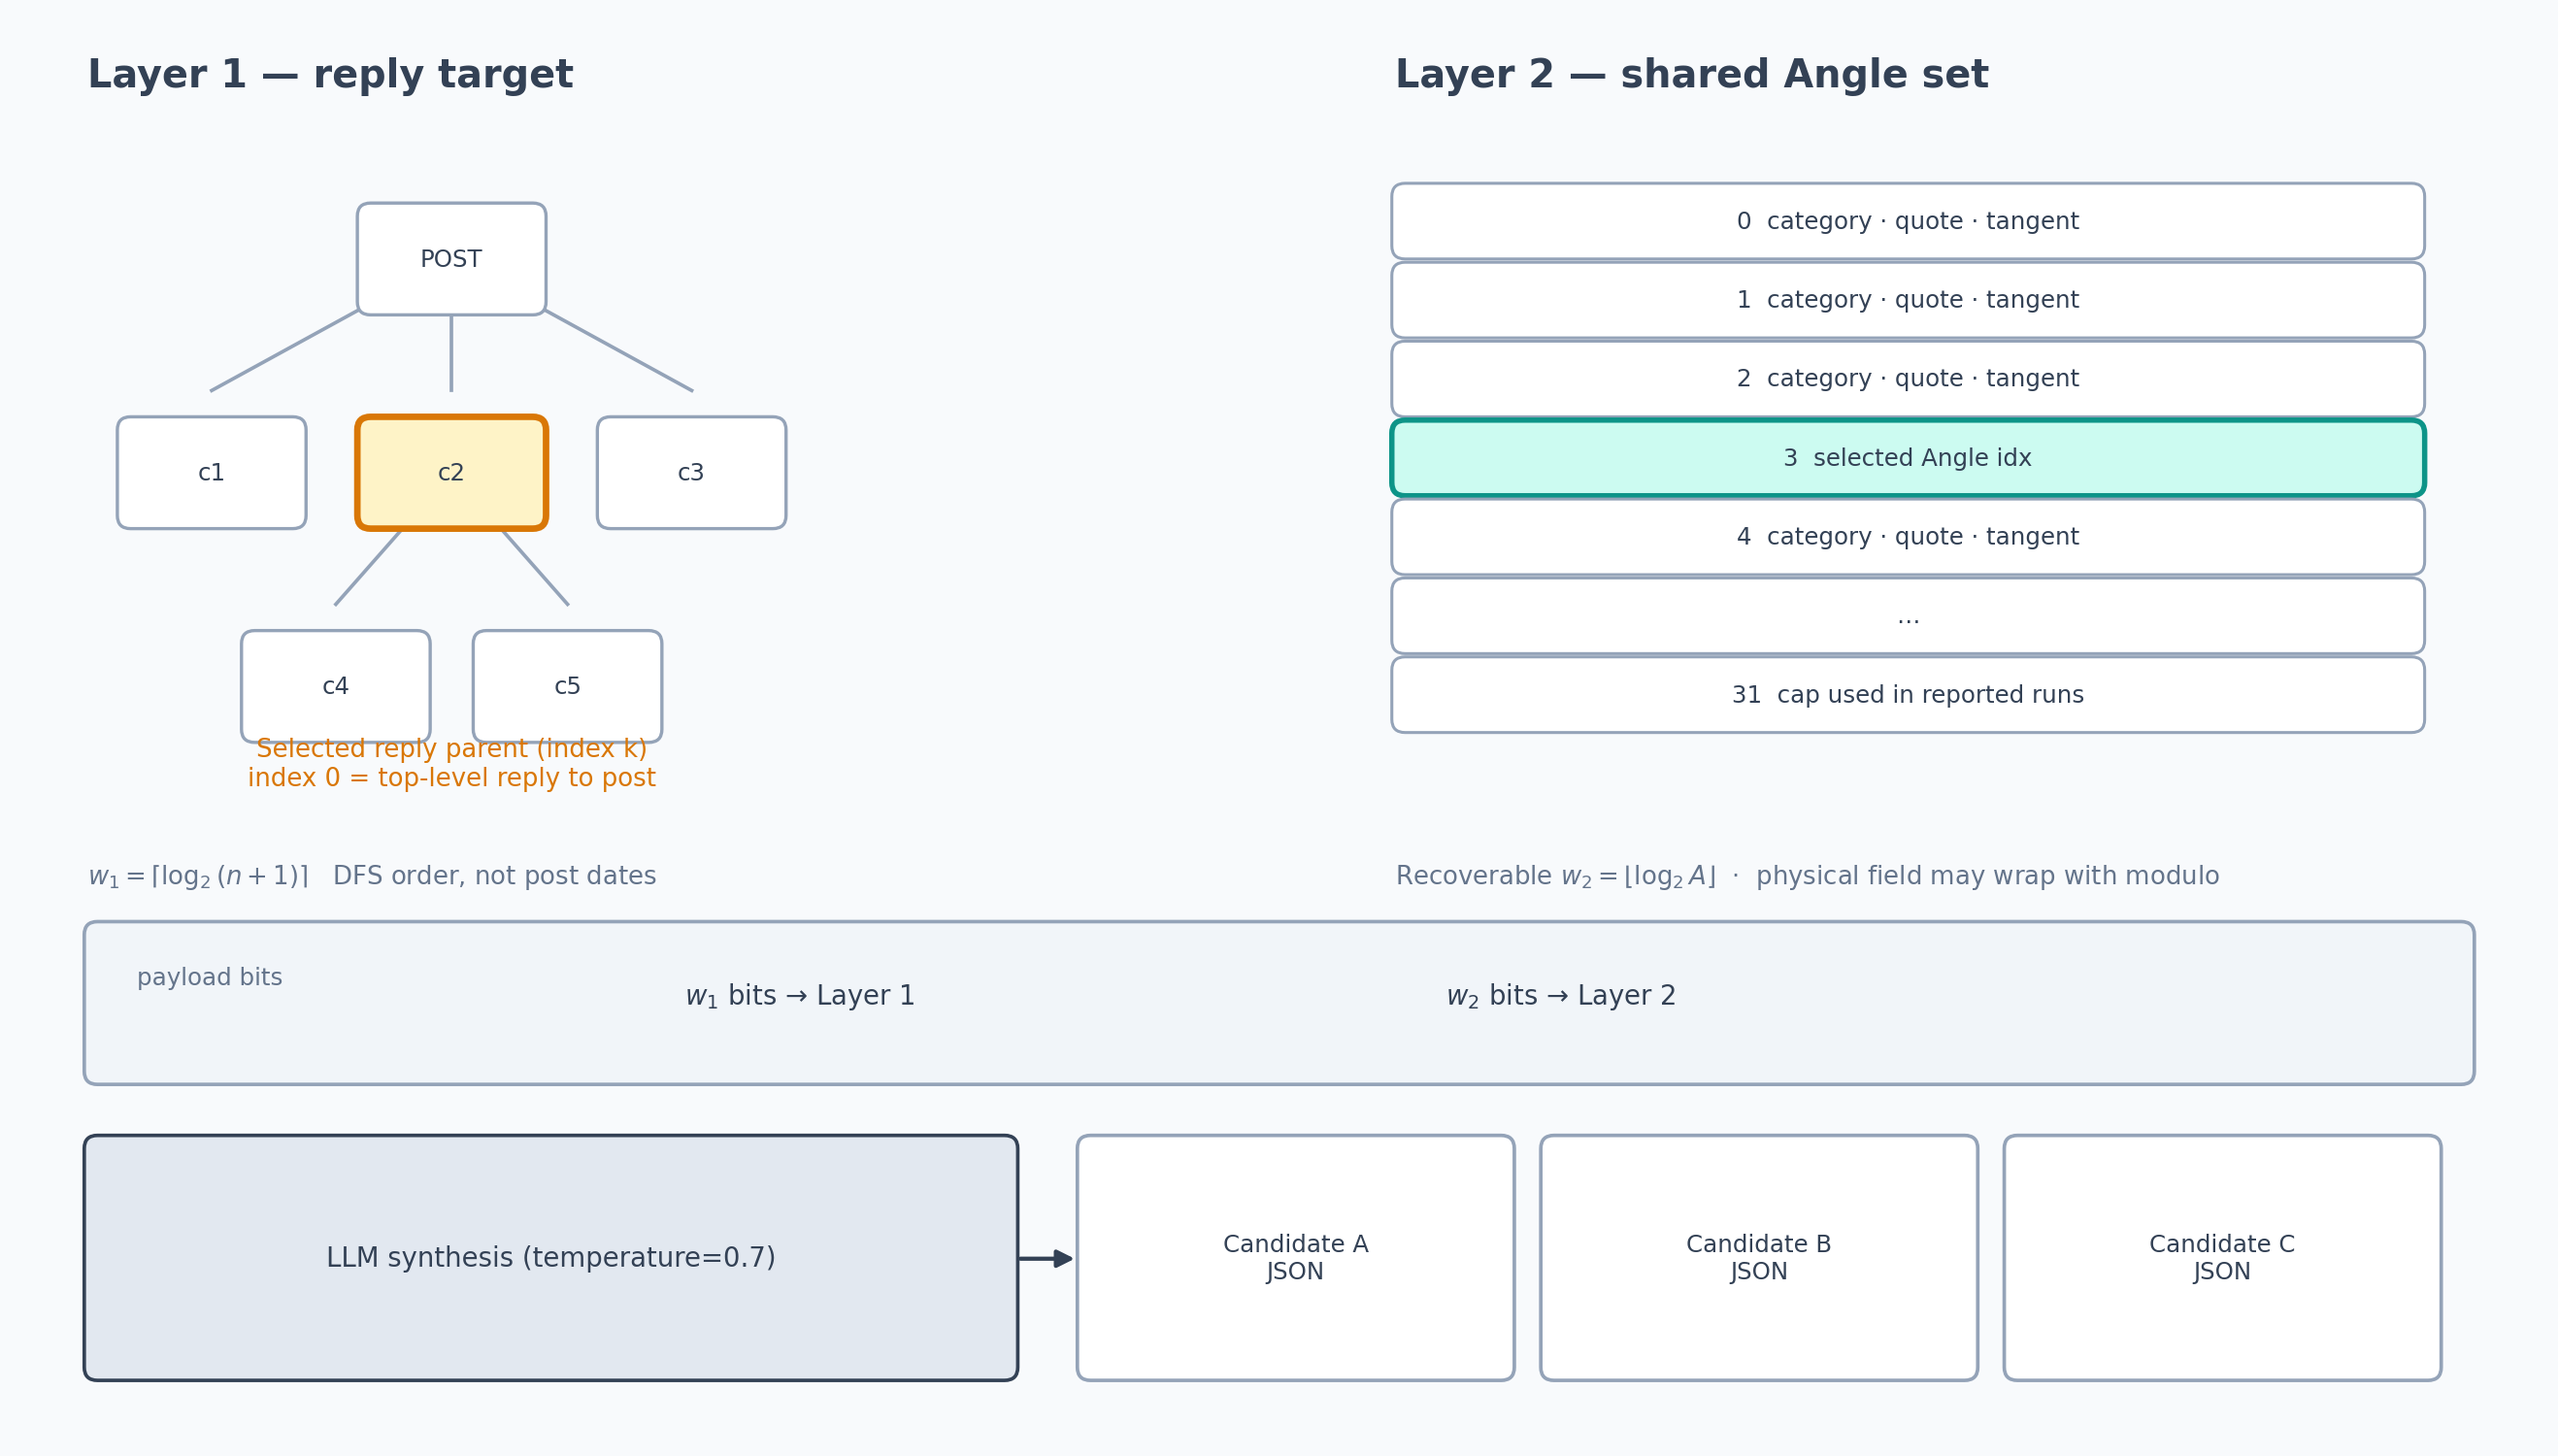
\includegraphics[width=\textwidth,height=0.65\textheight,keepaspectratio]{figures/two_layer_embedding}
	\caption{التضمين ثنائي الطبقة: تختار الطبقة الأولى موضع الرد في سلسلة مسطحة حتميًا، وتختار الطبقة الثانية وجهة نظر من مجموعة مشتركة يعاد بناؤها حتميًا؛ وتوجه البتات المدمجة عملية التوليد.}
	\label{fig:two-layer}
\end{figure*}

\subsubsection{الطبقة الأولى: التضمين المكاني، أي استهداف الرد}
\label{sec:layer1}
تحدد طبقة التضمين الأولى \textit{الموضع البنيوي} للمساهمة الإخفائية.
\begin{enumerate}
    \item يسطح النظام شجرة التعليقات المتداخلة بمسار حتمي من نوع العمق أولًا.
    \item يحصل كل هدف رد على فهرس بعرض ثابت، غير أن $\lfloor\log_2 C\rfloor$ بتًا فقط منه مضمونة الاسترجاع، حيث $C$ عدد الأهداف القابلة للاختيار (يوضح القسم~\ref{sec:channel-widths} لماذا لا يؤمن استخدام عرض الفهرس الخام مباشرة).
    \item يقابل الفهرس 0 ردًا عالي المستوى على المنشور، بينما يختار أي فهرس آخر تعليقًا محددًا، ويعيد المستقبل بناء سلسلة آبائه الكاملة بالصعود في السلسلة.
\end{enumerate}

\subsubsection{الطبقة الثانية: التضمين القائم على القصد، أي اختيار وجهة النظر}
\label{sec:layer2}
تحدد الطبقة الثانية \textit{القصد التواصلي}.
\begin{enumerate}
    \item \textbf{إعادة بناء مجموعة وجهات النظر:} باستخدام سلسلة المعالجة الحتمية، قسم~\ref{sec:search_determinism}، ولقطة السلسلة المرشحة، يعيد الطرفان توليد القائمة المرتبة نفسها من وجهات النظر المرشحة، حيث توصف كل وجهة نظر بوسم فئة، واقتباس مصدر، وحقل \textit{وجهة نظر} يمثل الاتجاه الموضوعي.
    \item \textbf{المقابلة الديناميكية للبتات:} تسند إلى القائمة المسطحة قيم \texttt{idx} متتالية، فيكون العرض القابل للاسترجاع $\lfloor\log_2 A\rfloor$ بتًا لعدد وجهات نظر متاحة $A$ -- وينطبق هنا التمييز نفسه بين العرض الفعلي والعرض القابل للاسترجاع من القسم~\ref{sec:channel-widths}، مع إحلال $A$ محل $C$.
    \item \textbf{اختيار وجهة النظر:} تقابل بتات الحمولة المناسبة فهرس وجهة نظر محددًا. وأثناء التوليد، تقرن وجهة النظر المختارة بسياق الرد ومقتطفات البحث ذات الصلة لإنتاج رد حامل معقول.
\end{enumerate}

\subsubsection{عرض القنوات وترتيب استهلاك البتات}
\label{sec:channel-widths}
تسحب الطبقتان كلتاهما من مقدمة السلسلة المضغوطة نفسها التي أنتجها القسم~\ref{sec:compression}: تستهلك الطبقة الأولى أول $w_1$ بتًا، وتستهلك الطبقة الثانية $w_2$ بتًا تليها. ويجب التمييز بين مفهومين للعرض، فالخلط بينهما هو أشيع طريقة للمبالغة في تقدير سعة هذه القناة.

أما \textit{العروض الفعلية} فهي أحجام الحقول المكتوبة فعلًا: $w_1=W(n)$ لسلسلة فيها $n$ تعليقًا، لأن أهداف الرد $C=n+1$ تفهرس من $0$، أي ردًا عالي المستوى على المنشور، حتى $n$؛ و$w_2=W(A-1)$ لعدد وجهات نظر مسطحة $A$. وحين يتجاوز العدد الصحيح المقروء من البتات أكبر خيار صالح، وهو أمر ممكن كلما لم يكن عدد الخيارات قوة للعدد 2، يرد المرمز القيمة بباقي القسمة على عدد الخيارات. فينجح التوليد دائمًا، لكن عدة أنماط بتات تنهار على اختيار مرصود واحد، فلا تكون تلك الأنماط قابلة للعكس.

وأما \textit{العروض القابلة للاسترجاع} فتستبعد هذا التداخل بالضبط: $\lfloor\log_2 C\rfloor$ و$\lfloor\log_2 A\rfloor$. ويقصر مسار التضمين الخالي من الفقد كل حقل على عرضه القابل للاسترجاع، ثم يعيد ترميز القيمة بالعرض الفعلي، وهو ما يجعل المقابلة من البتات إلى الاختيارات المرصودة متباينة بحكم البناء. وتستند دعاوى السعة في القسم~\ref{sec:evaluation} إلى العروض القابلة للاسترجاع.

ولاستهلاك مقدمة السلسلة، لا وحدة محددة الحدود ذاتيًا -- أي تعلن طولها بنفسها مسبقًا -- نتيجتان. أولاهما أن أول بت تقرؤه الطبقة الأولى هو راية نمط الضاغط، فالطبقتان تعتمدان على مخرج الضاغط لا على السلسلة ومجموعة وجهات النظر وحدهما. وثانيتهما أن المنشور الواحد يحمل $w_1+w_2$ بتًا \textit{فعليًا} بالضبط (القسم~\ref{sec:channel-widths})؛ فتخلف الحمولة الأطول فائضًا يبلغ عنه المرمز بوصفه غير مضمن بدلًا من إسقاطه صامتًا. ولذلك يعتمد استرجاع حمولة تتجاوز سعة منشور واحد من تعليق مرئي واحد على بيانات وصفية من جانب المرسل، أي الاسترجاع المدعوم بالتدقيق، ويذكر بهذه الصفة في التقييم. أما الاسترجاع الأعمى على نطاق أوسع فهو مهمة بروتوكول تعدد الأطر الموصوف تاليًا.

\subsection{النقل متعدد الأطر}
\label{sec:multiframe}
لحمل حمولات تتجاوز سعة منشور واحد، يوزع المرسل سلسلة البتات على عدة أطر، والإطار هو تعليق رد واحد يوضع تحت منشور واحد (وقد يستضيف المنشور الواحد أكثر من إطار -- انظر أدناه).

تحمى الحمولة أولًا كما سبق، ثم تضغط مقابل قاموس \textit{فارغ}، وهو ما يعطي بحكم قاعدة التراجع في القسم~\ref{sec:compression} النمط القياسي دائمًا: راية \EN{\texttt{0}} تتبعها بتات \EN{UTF-8} الخام. ولا يستخدم ضغط القاموس هنا عن قصد، لأن الأطر تمتد على عدة منشورات ولا يشترك فيها جميعًا قاموس جلسة واحد.

ثم تسبق البتات الناتجة بترويسة تحكم محددة الحدود ذاتيًا مبنية من ترميزي \EN{Elias-gamma}: عدد الأطر $F$، ثم طول الحمولة بالبتات، بحيث يعرف المستقبل المقدارين قبل قراءة أي بت من الحمولة. واختير \EN{Elias-gamma} على ترويسة ثابتة العرض لأن الترويسة نفسها تحمل عبر القناة الشحيحة ذاتها.

بعد ذلك تسند الأطر إلى خانات، إذ يسهم كل منشور بعدد مضبوط من الخانات سعة كل منها هي السعة القابلة للاسترجاع في القسم~\ref{sec:channel-widths}. ولأن طول الترويسة يتعلق بـ$F$ بينما تتعلق السعة المتاحة بعدد الخانات المستخدمة، يبحث المخطط تصاعديًا من $F=1$ عن أصغر عدد أطر تكفي فيه سعات الخانات الأولى $F$ للسلسلة المبنية بالقيمة $F$ نفسها. ويحشى الإطار الأخير بأصفار حتى عرض خانته؛ وعلى جانب الاستقبال يرفض المحلل أي سلسلة يخالف فيها عدد الأطر المصرح به العدد المرصود أو لا تكون فيها الحشوة أصفارًا كلها، وهو ما يحول القراءة غير المتزامنة إلى فشل نظيف بدلًا من حمولة خاطئة معقولة.

يفترض الوصف أعلاه مجموعة وجهات نظر ثابتة تتشاركها كل الأطر (المعاين على مستوى المنشور). أما تحت المعاين \textit{المرجح بالسياق} -- وهو النمط المستخدم لإنتاج النتائج المذكورة في القسم~\ref{sec:evaluation} -- فتتعلق مجموعة وجهات النظر بالتعليق الأب المختار، فيعمل المخطط على مرحلتين لكل إطار: يحل أولًا بتات اختيار الأب، ثم يعيد توليد مجموعة وجهات النظر مشروطة بذلك الأب، وعندئذ فقط يقيس عرض حقل وجهة النظر للبتات المتبقية.

\subsection{التوليد والتحقق}
بعد اختيار السياق الهدف ووجهة النظر المختارة، يبدأ المرسل عملية توليد النص الحامل.
\begin{itemize}
    \item \textbf{التوليد:} ينتج نموذج لغة توليدي قابل للضبط، يعمل عند حرارة غير صفرية، مجموعة صغيرة ثابتة من الردود القصيرة الملائمة للسلسلة على هيئة قائمة \EN{JSON} من سلاسل غير فارغة. ويشترط الموجه على بيانات المنشور، وسلسلة التعليقات المختارة، ووجهة النظر المختارة، ومقتطفات البحث ذات الصلة.
    \item \textbf{حلقة التحقق:} قبل تثبيت النص المُوَرّى في القناة العامة، ينفذ المرسل \textit{محاكاة محلية لفك الترميز} للتحقق من بقاء النص المولد قابلًا للاسترجاع.
    \item \textbf{التحسين التكراري:} إذا فشلت المحاكاة في استرجاع وجهة النظر المقصودة، يعيد المرسل تنفيذ التوليد دون تغيير معاملات التضمين. وتضمن الحرارة غير الصفرية تنوع المخرجات، بينما تقيد حلقة الإعادة بميزانية محاولات ثابتة.
\end{itemize}
يلخص الشكل~\ref{fig:verify-decode} تحقق جانب المرسل واسترجاع جانب المستقبل.

\begin{figure*}[t]
	\centering
	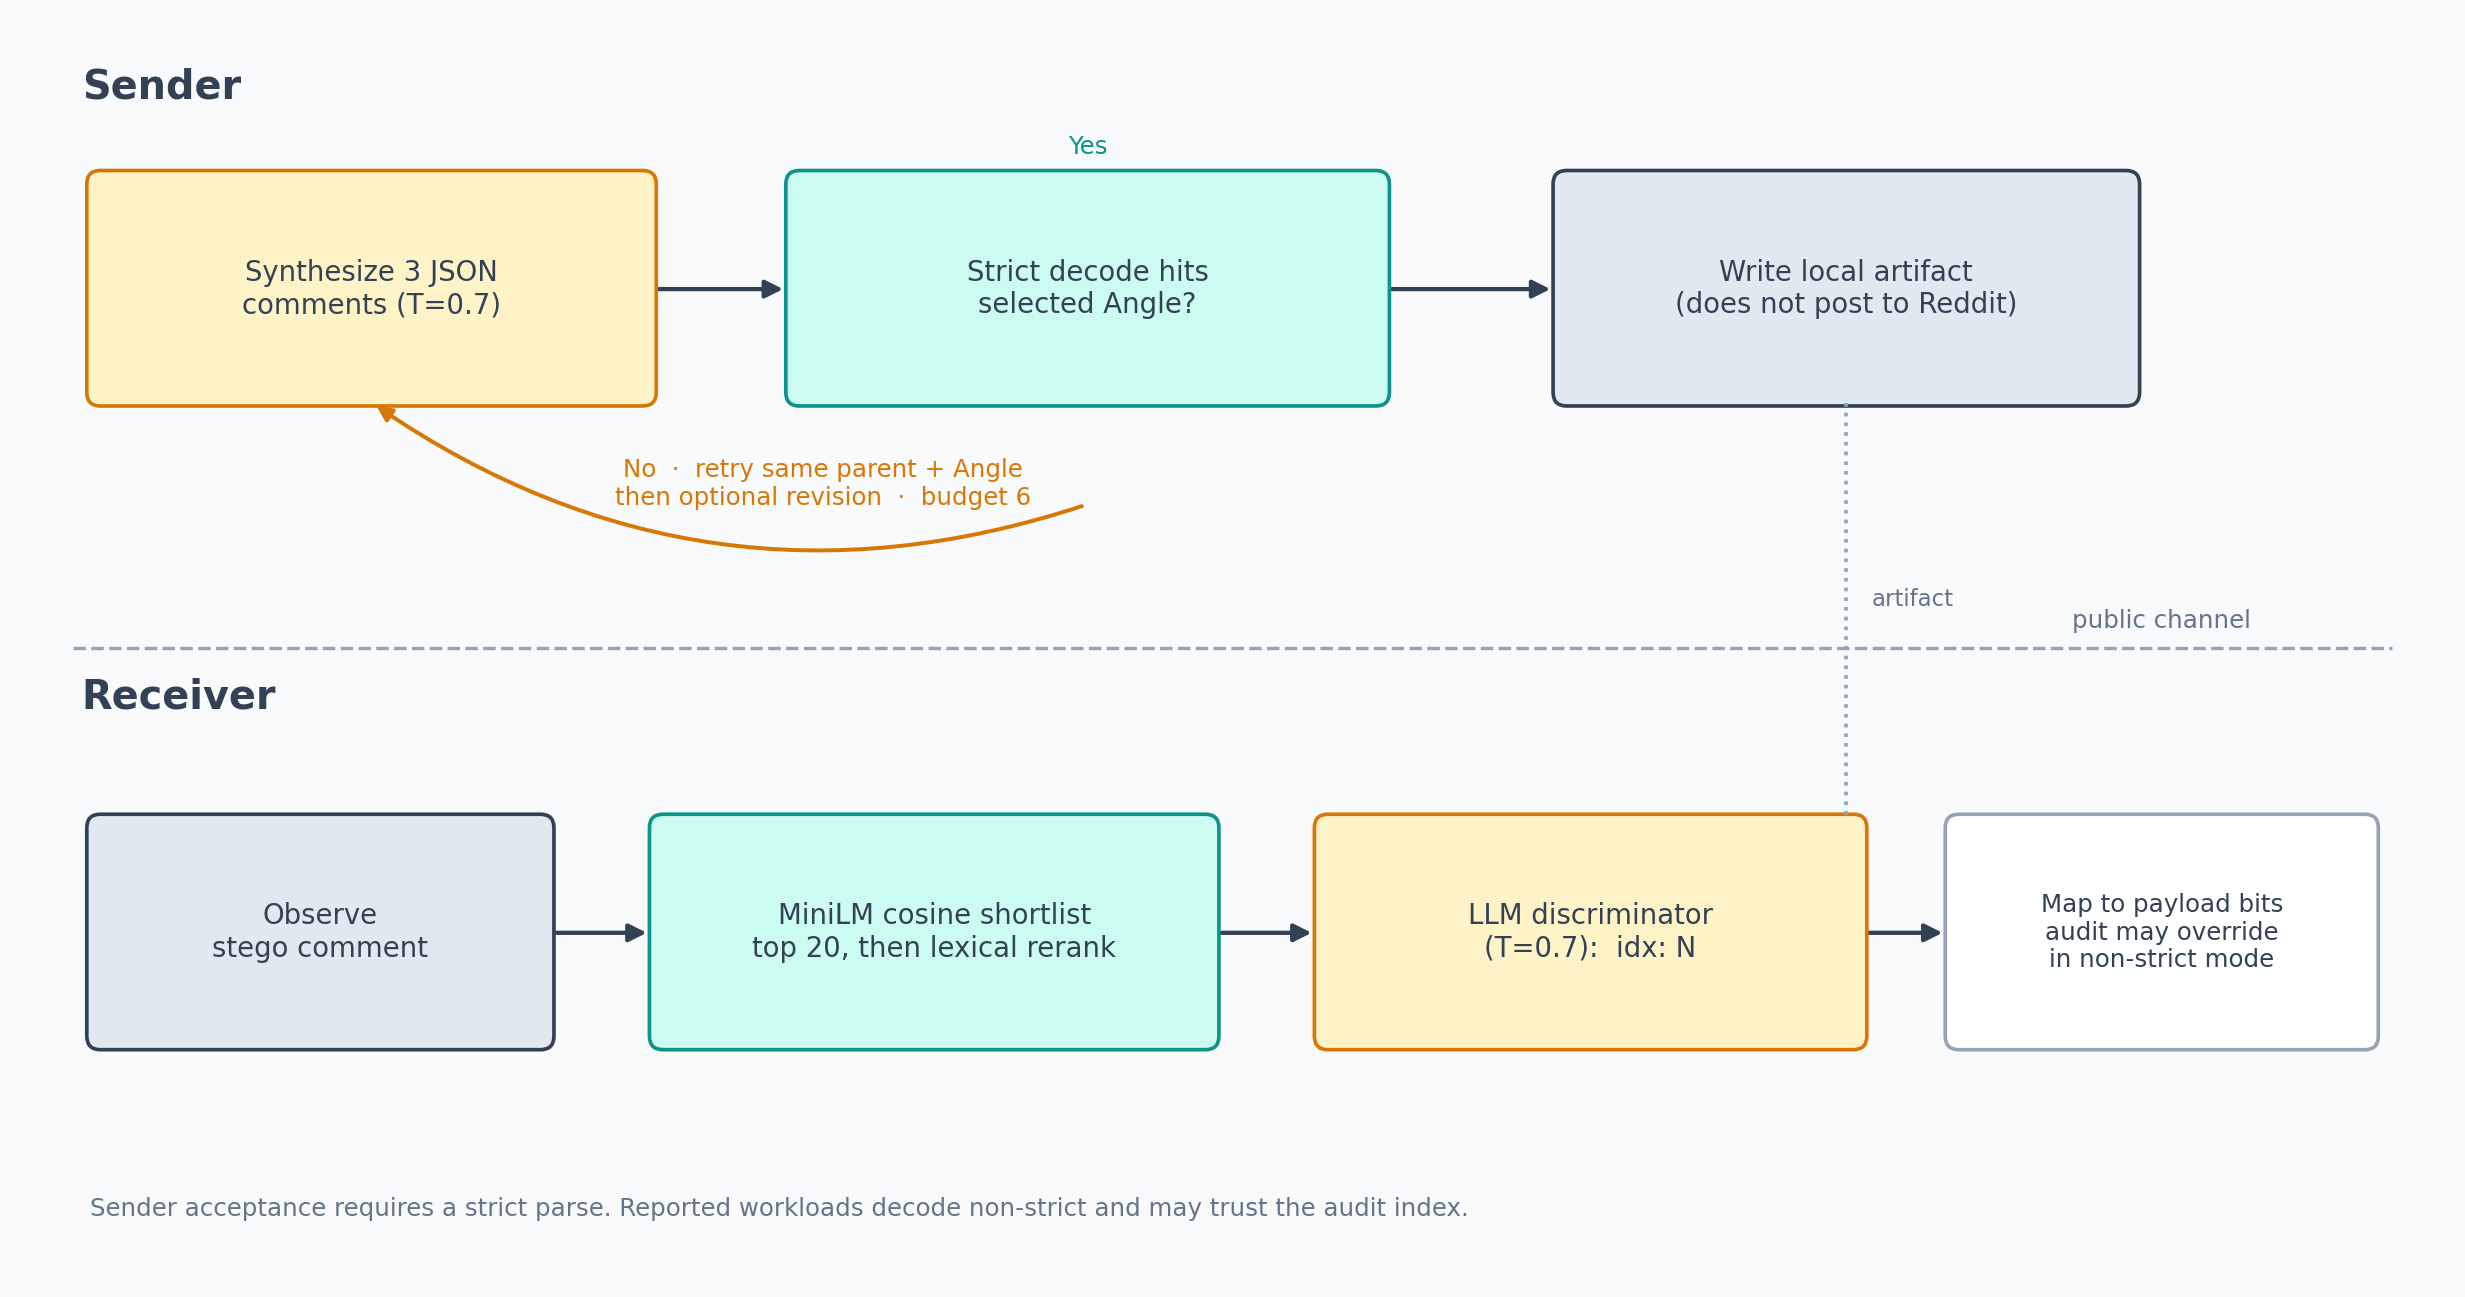
\includegraphics[width=\textwidth,height=0.62\textheight,keepaspectratio]{figures/verify_and_decode_flow}
	\caption{يعيد تحقق جانب المرسل محاولة التوليد حتى ينجح فك الترميز؛ ويسترجع المستقبل الطبقة الثانية عبر قائمة دلالية مختصرة وخطوة تحديد تمييزية.}
	\label{fig:verify-decode}
\end{figure*}

\subsection{فك الترميز واسترجاع القصد}
لاسترجاع القصد المخفي في الطبقة الثانية، يعيد المستقبل أولًا بناء سياق ما قبل المرسل إعادةً قابلة للحتمية عند تطابق المدخلات والإعدادات، ثم يفك اختيار وجهة النظر من الرد المرئي:
\begin{enumerate}
    \item \textbf{إعادة بناء السياق:} يحدد المستقبل التعليق المُوَرّى المرشح، ويحذفه من السلسلة، ويطبق حد الزمن $t_{publish} - T_{sync}$، ثم يعيد تشغيل المعالجة الحتمية، بما في ذلك تطبيع الروابط والبحث وتوليد وجهات النظر، لإنتاج قائمة وجهات النظر المرتبة نفسها.
    \item \textbf{الترشيح الدلالي:} يقصر نموذج تشابه دلالي القائمة على أفضل $N$ وجهة نظر توافق أوصافها النصية الرد الإخفائي المرصود.
    \item \textbf{التحديد التمييزي:} ينفذ موجه تحديد قابلًا للتثبيت عند \texttt{temperature=0} على المرشحين المختصرين لإرجاع فهرس وجهة النظر الأرجح:
          \begin{quote}
              \textit{``حدد وجهة النظر المحددة من المرشحين المعطاة... وأعد الفهرس فقط.''}
          \end{quote}
\end{enumerate}
وإذا أعاد المميز رتبة تبدأ من 1 بدلًا من الفهرس الخام، يقابلها خط المعالجة مع القائمة المختصرة؛ وإلا يعود إلى أعلى تطابق دلالي. وحرارة فك الترميز وحجم القائمة المختصرة قابلان للضبط، لذلك لا تكون هذه المرحلة حتمية بطبيعتها. ويشير \textbf{الاسترجاع} هنا إلى النتيجة العامة لاستعادة الحمولة، بينما يشير \textbf{فك الترميز} إلى عملية تحويل الاختيار المرصود إلى فهرس أو بتات. وقد يكون الاسترجاع خالصًا عبر قناة الانتقاء فقط عندما يعيد المستقبل بناء المدخلات وعقد فك الترميز نفسها، أو مدعومًا بالتدقيق عند توفر بيانات وصفية من المرسل. وبالاقتران مع الطبقة الأولى، أي استهداف الرد، تعيد الفهارس المسترجعة بناء بتات الانتقاء.

\paragraph{ملاحظة اصطلاحية.}
تُستخدم ``وجهة النظر'' بوصفها اسمًا لكائن البيانات الدلالي، لا بمعناها الهندسي؛ وتتضمن الفئة واقتباس المصدر والاتجاه الموضوعي. وتُستخدم ``قناة الانتقاء'' للدلالة على القناة التي تحمل الحمولة عبر اختيار حالات منفصلة، بينما يقتصر وصف ``حتمي'' على المراحل التي تثبت مدخلاتها وإعدادات النموذج والواجهة الخلفية. أما قائمة المرشحين فتسمى ``القائمة المختصرة للمرشحين''، وتسمى العملية الإحصائية لاستعادة الفهرس ``التحديد'' لا ``الاسترجاع''.
\FloatBarrier
